\chapter{This Land Is My Land}

These companion notes follow Michael Sandel's fourth lecture in the \textit{Justice} course, as curated in the LazyLearn track by LazyingArt LLC. The lecture is organized as a controlled reversal. At first Locke looks like a powerful ally of libertarianism: he affirms natural rights to life, liberty, and property, and he insists that these rights do not depend on government for their existence. But as Sandel unfolds the argument, that first impression becomes harder to sustain. We move from natural rights to the state of nature, from the state of nature to property, from property to consent, and finally to the question that the lecture leaves open: what, exactly, can consent justify?

\section{Locke as the Apparent Libertarian Ally}

Sandel opens with a clean and strategic framing. On the face of it, Locke is a powerful ally of the libertarian. He believes that there are fundamental individual rights that no government may override, not even a representative or democratically elected one. The rights at issue are the familiar Lockean triad:
\begin{equation}
R_{\mathrm{nat}}=\{\text{life},\ \text{liberty},\ \text{property}\}.
\end{equation}

The point is not merely that these rights are important. It is that they are natural. In particular, Locke's right to property is not treated as the product of legislation:
\begin{equation}
\text{property is a natural right}
\Longrightarrow
\text{property is pre-political in principle.}
\end{equation}

That is the lecture's opening pressure point. If property is not simply created by law, then we must be able to say what it means before legislatures, courts, and governments arrive on the scene. Sandel therefore moves immediately to the thought experiment that makes Locke's whole view intelligible: the state of nature.

\section{State of Nature: Liberty, Not License}

The state of nature is not introduced as a chaotic historical episode. It is introduced as a conceptual setting in which we can ask what a natural right would be if there were no enacted law to define or enforce it. Locke says that the state of nature is a state of liberty, and Sandel is careful to add the corresponding claim that human beings in that condition are free and equal. There is no natural hierarchy: some are not born kings while others are born serfs.

But the lecture's first real distinction appears as soon as that point is made:
\begin{equation}
\text{State of Nature}=\text{Liberty}\neq \text{License}.
\end{equation}

This is not merely a verbal refinement. It is the first formal obstacle in the lecture. If the state of nature is a state of liberty, why is it not a state of unrestricted permission? Sandel answers: because even in the state of nature there is a law, though not a humanly enacted one. There is a law of nature.

\subsection{Question \& Answer}

\paragraph{Question.} If we are free and equal in the state of nature, why are we not free to do whatever we want?

\paragraph{Answer.} Because freedom here means the absence of natural masters, not the absence of all norm. The law of nature constrains action before there is legislation. Sandel compresses the constraint into two paired prohibitions:
\begin{equation}
\neg \text{Alienate}\big(R_{\mathrm{nat}}(x)\big)
\qquad\text{and}\qquad
\neg \text{Violate}\big(R_{\mathrm{nat}}(y)\big).
\end{equation}

In plain language, we may neither give up our own natural rights nor take those of another. That is why the lecture can say, without contradiction, that we are free and yet are not free to kill, enslave, or subject either ourselves or others to arbitrary absolute power. The state of nature is morally structured from the start.

\section{Unalienable Rights and Their Two Foundations}

Once liberty has been distinguished from license, Sandel asks the next question in the lecture's own order: where does the constraint come from? Locke offers two answers, and Sandel preserves their sequence.

The first answer is theological. Human beings are the workmanship of God. So the reason we cannot simply dispose of our lives and liberties at will is that they are not fully ours in the first place. As a compact summary,
\begin{equation}
\text{God's prior property right in us}\succ \text{our discretionary power over ourselves}.
\end{equation}

This is already enough to explain why self-sale into slavery, self-destruction, or the surrender of arbitrary power over oneself is forbidden. But Sandel does not allow the argument to rest there. He immediately asks what Locke can say to those who do not begin from theology, and that turns the lecture toward reason.

The second answer is rational rather than theological:
\begin{align}
\text{Reason} &= \text{Law of Nature},\\
\forall x\neq y,\quad x &\text{ ought not harm } y \text{ in life, health, liberty, or possessions.}
\end{align}

We should read this as a compact summary of the lecture, not as a literal line of formal notation in Locke. Its force is nonetheless exact. Proper reflection on what it means to be free leads us away from the idea that freedom is just doing whatever we want and toward the idea of a law that binds equals as equals.

This is also where Sandel introduces the paradox of unalienability. The airline-ticket analogy does real philosophical work. A non-transferable ticket is, in one familiar sense, less fully mine because I cannot sell or trade it. But a right can be unalienable in a deeper sense: so essentially mine that even I cannot give it away. That is Locke's sense of the term, and Sandel explicitly connects it to Jefferson's use of unalienable rights in the Declaration of Independence.

At this point in the lecture Locke begins to move away from the libertarian. If rights are truly natural, then taking them seriously does not yield absolute self-ownership. It yields the claim that some of the things most truly ours are precisely the things we may not dispose of at will.

\section{Property Before Government: From Person to Labor to Land}

And yet the lecture does not stay there. Sandel now turns to the issue on which Locke begins to look like a plausible libertarian ally again: private property. The key question is not whether life and liberty can be natural rights. It is whether private property can arise even before government exists to define or enforce it.

Locke's answer in Section 27 starts from the person and moves outward:
\begin{equation}
\text{property in person}\to \text{property in labor}\to \text{mix labor with unowned things}\to \text{private property}.
\end{equation}

This is the central constructive chain of the lecture. The important thing is that Sandel unfolds it step by step rather than presenting it as a slogan.

\paragraph{Worked derivation.}
\begin{enumerate}
\item Every person has a property in his own person.
\item The labor of his body and the work of his hands are therefore properly his.
\item Let \(o\) be something unowned and left in common.
\item Once labor that is already mine is mixed with \(o\), the object is no longer simply where nature left it.
\item Because the labor is unquestionably the laborer's own, what is joined to it may become the laborer's property.
\end{enumerate}

In schematic notation we may write:
\begin{equation}
o\in U,\qquad \operatorname{Mix}(L_x,o)\Longrightarrow o\in P_x,
\end{equation}
where \(U\) is the common stock of unowned things, \(L_x\) the labor of person \(x\), and \(P_x\) what belongs to \(x\). This is cautious editorial shorthand, but it captures the structure Sandel is extracting from Locke.

\paragraph{A worked example.}
Suppose an apple lies in the common stock \(U\). If person \(x\) picks it, then the apple is no longer merely where nature left it. It has been joined to labor that already belongs to \(x\). In that simple case, the apple may become \(x\)'s property.

But Locke wants more than the apple case. He wants the stronger land case. If a parcel is tilled, planted, improved, cultivated, and enclosed, then the claim extends beyond the crop to the land itself:
\begin{equation}
\text{till}+\text{plant}+\text{improve}+\text{cultivate}
\Longrightarrow
\text{property not only in crop but in land}.
\end{equation}

This is why the argument is controversial. The move from apples and acorns to land is not a minor extension. It is a qualitative increase in the strength of the claim.

Locke's argument is not, however, unrestricted. Sandel emphasizes the proviso:
\begin{equation}
\text{valid appropriation}\Longrightarrow \text{``enough and as good'' left for others.}
\end{equation}

So the lecture's constructive chain has a clear internal discipline. Labor can ground appropriation, but appropriation is valid only under a condition that keeps the common world from being exhausted by a first claimant.

\subsection{Question \& Answer}

\paragraph{Question.} How can private property arise before government or consent?

\paragraph{Answer.} Locke's answer is that the original act of appropriation does not require prior agreement. The relevant moral bridge is labor. We begin with property in the person, pass from person to labor, and then treat labor mixed with the unowned as sufficient to generate ownership. Consent enters later, not to create the very possibility of property, but to create the political order in which property is defined, stabilized, and adjudicated.

\section{Testing Locke's Property Argument: Patents, Colonization, and Common Use}

Sandel does not let the labor theory remain an elegant abstraction. He tests it twice, first with a modern case and then with a historical objection.

The modern case is the dispute over drug patents during the AIDS crisis in South Africa. Western governments and pharmaceutical companies argue that research, ingenuity, and investment create a legitimate claim over the resulting drug. The South African government replies that generic versions could save lives at a tiny fraction of the cost. The case matters in the lecture because it keeps alive the intuition that labor or creation can generate ownership while also showing that property claims do not float free from human consequences.

Sandel then makes a striking suggestion. Among nations, where there is no single settled law of patents and property, the dispute looks in one respect like a frontier case, almost a last remnant of the state of nature. The point is not that intellectual property works exactly like land appropriation. It is that before settled rules exist, the question of property remains morally and politically open.

From there the lecture turns to the classroom challenge about Native Americans and European settlement. Rochelle's objection is the crucial one: if Locke's argument is sound, then it may justify colonial appropriation; if it is unsound, then it functions as a rationalization for it. Sandel deliberately sharpens the dilemma rather than softening it.

The replies stay within Locke's framework. Dan notes that use itself may count as labor. If picking an acorn or killing a buffalo is enough to ground a claim, then Native American patterns of use may already amount to a property claim. Fang adds the second pressure point: common use and the proviso. If land is used in common, and if valid appropriation requires enough and as good to remain for others, then easy colonial enclosure becomes harder to defend.

Sandel does not tie this up neatly, and he should not. The point of the exchange is to show that Locke's account of original acquisition is strongest precisely where it becomes morally most suspect. That is the point at which the lecture turns. If property is natural rather than conventional, what becomes of that right once we enter society? That question leads from property to consent.

\section{Consent as the Second Big Idea}

After a brief editorial reset in the broadcast, Sandel explicitly says that consent is Locke's second big idea. He even reminds us that consent has been hovering over the course from the beginning: it appeared in the discussion of pushing the fat man, and again in the discussion of the cabin boy. So by the time we arrive at Locke, consent is already familiar. The philosophical work of the lecture is to make it strange again.

To do that, Sandel returns us to the state of nature. Why leave it at all? Locke's answer is not that the state of nature lacks rights. It is that the enjoyment of those rights is insecure because everyone may enforce the law of nature for himself or herself. Everyone is an executor of the state of nature, and because each person becomes judge in his or her own case, punishment overshoots.

The lecture's transition is therefore:
\begin{equation}
\text{everyone enforces law of nature}
\to
\text{punishment overshoots}
\to
\text{insecurity}
\to
\text{consent to civil society}.
\end{equation}

What is surrendered when we consent is not the rights themselves but the private power to enforce them:
\begin{equation}
\text{consent}\Longrightarrow \text{surrender private enforcement power},
\qquad
\text{not}\Longrightarrow \text{surrender natural rights}.
\end{equation}

\begin{figure}[h]
\centering
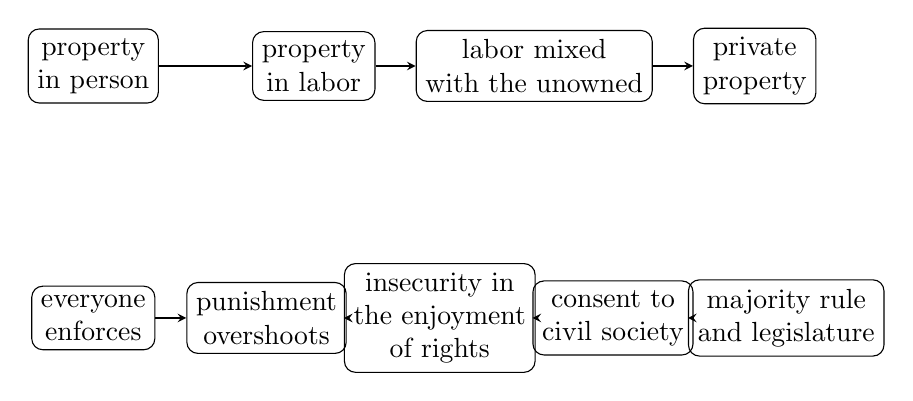
\begin{tikzpicture}[>=stealth]
\node[draw, rounded corners, align=center] (p1) at (0,1.7) {property\\in person};
\node[draw, rounded corners, align=center] (p2) at (2.8,1.7) {property\\in labor};
\node[draw, rounded corners, align=center] (p3) at (5.6,1.7) {labor mixed\\with the unowned};
\node[draw, rounded corners, align=center] (p4) at (8.4,1.7) {private\\property};

\draw[->] (p1)--(p2);
\draw[->] (p2)--(p3);
\draw[->] (p3)--(p4);

\node[draw, rounded corners, align=center] (c1) at (0,-1.5) {everyone\\enforces};
\node[draw, rounded corners, align=center] (c2) at (2.2,-1.5) {punishment\\overshoots};
\node[draw, rounded corners, align=center] (c3) at (4.4,-1.5) {insecurity in\\the enjoyment\\of rights};
\node[draw, rounded corners, align=center] (c4) at (6.6,-1.5) {consent to\\civil society};
\node[draw, rounded corners, align=center] (c5) at (8.8,-1.5) {majority rule\\and legislature};

\draw[->] (c1)--(c2);
\draw[->] (c2)--(c3);
\draw[->] (c3)--(c4);
\draw[->] (c4)--(c5);
\end{tikzpicture}
\caption{A note-native reconstruction of the lecture's two central chains: appropriation through labor and the transition from private enforcement to civil society.}
\end{figure}

\subsection{Question \& Answer}

\paragraph{Question.} If natural rights remain in force, what exactly does consent authorize the majority to do?

\paragraph{Answer.} Consent authorizes the formation of a political community with law, legislature, and majority decision. It explains why we leave the state of nature and why we accept a standing authority in place of private enforcement. But it does not, by itself, explain how far that authority may go. Natural rights do not disappear when civil society begins, and that is why the lecture's second half takes the form of a puzzle rather than a simple vindication of majority rule.

\section{Taxation, Implied Consent, Conscription, and Locke's Limits}

Once civil society has been formed, Sandel presses the central question: what can the majority actually decide? At first Locke still seems friendly to libertarian hopes. If natural rights persist into civil society, then no parliament or legislature, however democratic, can legitimately violate them. Sandel deliberately lets that thought arise and then warns us not to be too quickly reassured.

The reason appears when he turns to Locke's own text on taxation. The sharp contrast is this:
\begin{equation}
\text{no taking of property without consent}
\qquad\text{vs.}\qquad
\text{his own consent}=\text{consent of the majority}.
\end{equation}

That is the pressure point of Sections 138 and 140. On the one hand, Locke says the legislature cannot take property without consent. On the other hand, when he explains taxation, he says that the relevant consent is majority consent, given directly or through representatives.

Sandel's reconstruction of the tension is especially careful here. Locke sometimes uses ``property'' broadly, almost as a global name for life, liberty, and property together. But he also says that in society people possess the goods that are theirs \emph{by the law of the community}. Hence the lecture's two-level distinction:
\begin{equation}
\text{property as an institution is natural},
\qquad
\text{what counts as mine is conventionally defined}.
\end{equation}

This is the point where the notes must not become too textbook-like. Sandel is not simply classifying property into two philosophical species. He is trying to make sense of an apparent contradiction in Locke. The institution of property limits government. But the specification of holdings is a matter for law. So the natural right is not a guarantee that each existing holding stands outside political definition. It is a guarantee against the destruction of the institution and against arbitrary seizure.

\subsection{Question \& Answer}

\paragraph{Question.} Can those who never explicitly consented still be bound by government and taxation?

\paragraph{Answer.} Locke seems forced toward a combination of collective and tacit consent. Collective consent enters when a people leaves the state of nature and agrees to majority rule. Tacit or implied consent enters when those born into an existing society accept its protections and continue to live under its institutions. Sandel does not present this as a clean solution. The student exchange is important precisely because it shows how weak the appeal to implied consent can sound once explicit agreement has disappeared.

The Nicola exchange makes the problem vivid. If someone obeys the law only for prudential reasons, because she does not want to be caught, then the moral force of consent seems to vanish. The reply offered in class is itself revealing: perhaps one cannot reject obligation while still taking the benefits of public order. One may try to return to the state of nature, but then one cannot keep driving on Mass Ave. That is not a decisive solution; it is evidence of how unstable the consent argument becomes at this point in the lecture.

The pressure then rises once more, from property to life itself.

\subsection{Question \& Answer}

\paragraph{Question.} If rights are unalienable, how can anyone be bound by taxation or conscription under majority rule?

\paragraph{Answer.} This is the deepest local obstacle in the lecture. If I cannot sell myself into slavery or consent to my own destruction, how can I be said to have consented to a law that taxes my property or may compel me into military service? Sandel's likely Lockean answer turns on one final distinction:
\begin{equation}
\text{arbitrary taking}=\text{illegitimate},
\qquad
\text{general non-arbitrary law}\neq \text{arbitrary taking}.
\end{equation}

On this reading, the true object of Locke's hostility is arbitrary power. What government may not do is single out Bill Gates to finance a war, or pick some particular citizen at pleasure to surrender his liberty or life. A general law, enacted through fair procedures and applied by standing rules, does not count as the same sort of violation. That is why Sandel takes Gokul's intervention so seriously: the difference between arbitrary choice and general law may be Locke's only escape.

This answer is intelligible, but it comes at a price. It means that unalienability does not yield absolute self-ownership, and it means that consent, once joined to general law, authorizes more than libertarians would like:
\begin{align}
\text{unalienable rights} &\Longrightarrow \text{self-ownership is not absolute},\\
\text{consent}+\text{general law} &\Longrightarrow \text{government may be less limited than libertarians hope}.
\end{align}

This is Sandel's final verdict on Locke as an ally of libertarianism. The libertarian is disappointed twice: first because natural rights are unalienable and therefore not fully disposable, and second because a legitimate government acting through non-arbitrary general law may still tax, regulate, and conscript.

The lecture then darkens one last time. Locke, the great theorist of consent, also produced a theory of private property that did not require consent at all. And when he says that ``all the world was America,'' Sandel invites us to hear the colonial background of the theory itself: enclosure, settlement, and war with Native Americans were not accidental illustrations. They may have been part of the work the theory was built to do.

\section{Summary}

Sandel begins by making Locke look like the libertarian's philosopher and ends by showing how unstable that appearance is. Natural rights are prior to government; the state of nature is a state of liberty but not license; and the law of nature constrains us first through divine workmanship and then through reason. Private property arises through the chain from person to labor to appropriation, but only under the proviso that enough and as good remain for others. Consent then enters as the mechanism by which we escape the insecurity of private enforcement and create civil society under majority rule.

But once taxation, implied consent, and conscription enter the picture, the theory changes shape. Locke limits arbitrary power, not government as such. That is why the lecture closes without full resolution. Consent plainly matters, but it does not explain everything, and it does not settle every burden that political life may impose. Sandel leaves us with that unfinished question and carries it forward to the next lecture, where the problem of consent moves from government to markets.